%% LyX 2.2.2 created this file.  For more info, see http://www.lyx.org/.
%% Do not edit unless you really know what you are doing.
\documentclass[english]{article}
\usepackage{mathptmx}
\usepackage{graphicx}
\usepackage{helvet}
\usepackage{courier}
\usepackage[T1]{fontenc}
\usepackage[latin9]{inputenc}
\usepackage{geometry}
\geometry{verbose,tmargin=2.5cm,bmargin=2.5cm,lmargin=2.5cm,rmargin=2.5cm,headheight=0cm,headsep=0cm}

\makeatletter
\@ifundefined{date}{}{\date{}}
\makeatother

\usepackage{babel}
\begin{document}

\title{The Programming Assignment Report Instructions\\
CSCE 221}
\maketitle
\begin{enumerate}
\item The description of an assignment problem.\\ \ \\

The purpose of this assignment was to create a C++ program that would allow a user to enter an expression with or without variables in infix form. The simple calculator would then evaluate the expression by utilizing a stack, a que, and postfix form. The stack and que also used the templated linked list class created in part 1. \\ \ \\

\item The description of data structures and algorithms used to solve the
problem.

\begin{enumerate}
\item Provide definitions of data structures by using Abstract Data Types
(ADTs) \\ \ \\

\begin{itemize}
  \item \textbf{Templated Doubly Linked List}: a sequence of nodes where each node contains a pointer to the previous node and next node in the sequence. Since it is templated, a variety of data types can be passed in.
  \item \textbf{Templated Linked Que:} a linear data structure where operations are performed based on first-in-first-out principle. Since it is templated, a variety of data types can be passed in.
  \item \textbf{Templated Linked Stack:} a linear data structure where the operations are performed based on last-in-first-out principle. Since it is templated, a variety of data types can be passed in.
  \item \textbf{String:} a container that holds an array of characters
  \item \textbf{Vector:} a container that can hold a variety of data types. Vector has several built in functions. Also provides bounds error checking.
  \item \textbf{Token:} a container that references a character to a value and/or weight.
\end{itemize} \ \\
\item Write about the ADTs implementation in C++. \\ \ \\

\begin{itemize}
  \item \textbf{Templated Doubly Linked List:} a list of doubly linked nodes. This data type has a constructor, copy constructor, desctructor, assignment operator, get first node pointer, get after last node, check if list is empty, return first node, return last node, insert a new node to the first position, remove the first node, insert a node in the last position, and remove last node. An overloaded output stream operator was used to display the all the nodes in the list. Finally everything was templated for use with a variety of data types.
  
  \item \textbf{Templated Linked Que:} contains a private doubly linked list variable. Functions include a constructor, copy constructor, destructor, return first element in que, check if que is empty, enqueue an item, dequeue an item, and an accessor function for the doubly linked list. An overloaded output stream operator was used to display the all the elements in the que. Finally everything was templated for use with a variety of data types.
  
  \item \textbf{Templated Linked Stack:} contains a private doubly linked list variable. Functions include a constructor, destructor, check if stack is empty, push an element to the stack, pop the top element of the stack, get top of the stack, and an accessor function for the doubly linked list. An overloaded output stream operator was used to display the all the elements in the stack. Finally everything was templated for use with a variety of data types.
  
  \item \textbf{String:} a constant char array
  
  \item \textbf{Vector:} a container that holds a list of elements that can be accessed using an iterator.
  
  \item \textbf{Token:} a struct that I created to hold an elements kind, value, and weight. Functions include a checker if element is an operator, checker if element is  an operand, checker if an element is a number, checker if an element is a variable, setter functions that sets the value, function to convert character to a double, and a get operator weight function.
\end{itemize} \ \\

\item Describe algorithms used to solve the problem.\\ \ \\
\begin{itemize}
  \item $Parser::toPostfix()$ this functions converts a vector of tokens in infix form to an equivalent postfix form. This functions iterates through each token in the vector. If the token is an operand, enqueue the operand until the next item is not an operand. If the token was an close parenthesis, pop items off the stack and enqueue that item until a left parenthesis is reached. If the token is an open parenthesis, push the item to the stack. if the token is a \#, pop an item of the stack and enqueue it until the stack is empty. Else, pop an item off the stack and enqueue it until the top item of the stack's weight is greater or equal to the tokens weight. Then enqueue the item. Finally, pop items off the stack and enqueue them until the stack is empty. Return the que.
  \item $Token::get\_operator\_weight()$ if kind is ( or ), weight is 1, if kind is $+$ or $-$, weight is 2, if kind is $*$ or $/$, weight is 3, if kind is \^{}, weight is 4, if kind is \~{}, weight is 5. Return weight
  \item $Evaluator::evaluate:$ taken in operator, v1, and v2. If operator is $+$, add v1 and v2. If operator is $-$, subtract v2 from v1. If operator is $*$, multiply v1 and v2. If operator is \^{}, raise v1 to the power of v2. If operator is $/$ and v2 is not 0, divide v1 by v2. If v2 was 0, throw a division by 0 exception.
  \item $Evaluator::getValue(): $ Set sign to be 1. While first item in que is not \#, if first item in que is \~{}, set sign to $-1$ and dequeue the item. If first item in que is a space, deqeue it. If first item inn que is an operand, deque the operand and string stream it into ss until a space is reached. Input the string stream into a double. Multiply the double by the current sign value. Set sign value to 1. Push the number to the stack. If the first item in the que is an operator, evaluate that operator while dequeueing (so many vowels in a row!) it along with the the two next popable items on the stack. Push that evaluated value to the stack. Else, return the last popped value of the stack.
\end{itemize} \ \\

\item Analyze the algorithms according to assignment requirements. \\ \ \\
\begin{itemize}
  \item $Parser::toPostfix(): \; O(n)$
  \item $Token::get\_operator\_weight(): \; O(1)$ 
  \item $Evaluator::evaluate: \; O(1)$
  \item $Evaluator::getValue(): \; O(n)$
\end{itemize} \ \\

\end{enumerate}
\item A C++ organization and implementation of the problem solution 
\begin{enumerate}
\item Provide a list and description of classes or interfaces used by a
program such as classes used to implement the data structures or exceptions.\\ \ \\

\begin{itemize}
  \item \textbf{Templated Linked Que:} contains a private doubly linked list variable. Functions include a constructor, copy constructor, destructor, return first element in que, check if que is empty, enqueue an item, dequeue an item, and an accessor function for the doubly linked list. An overloaded output stream operator was used to display the all the elements in the que. Finally everything was templated for use with a variety of data types.
    
    \item \textbf{Templated Linked Stack:} contains a private doubly linked list variable. Functions include a constructor, destructor, check if stack is empty, push an element to the stack, pop the top element of the stack, get top of the stack, and an accessor function for the doubly linked list. An overloaded output stream operator was used to display the all the elements in the stack. Finally everything was templated for use with a variety of data types.
\end{itemize} \ \\

\end{enumerate}
\item A user guide description how to navigate your program with the instructions
how to: 
\begin{enumerate}
\item compile the program: specify the directory and file names, etc.\\ \ \\
Make sure you are in the directory "~/Martinsen-Joseph-A3P3/Martinsen-Joseph-A3P3code/" \\
Compile the program with "make"
\item run the program: specify the name of an executable file. \\ \ \\
Run the program with "./run-main"
\pagebreak{}
\end{enumerate}
\item Specifications and description of input and output formats and files 
\begin{enumerate}
\item The type of files: keyboard, text files, etc (if applicable). \\ \ \\
No input or output files \\ \ \\

\item A file input format: when a program requires a sequence of input items,
specify the number of items per line or a line termination. Provide
a sample of a required input format. \\ \ \\
Not applicable

\item Discuss possible cases when your program could crash because of incorrect
input (a wrong file name, strings instead of a number, or such cases
when the program expects 10 items to read and it finds only 9.)\\ \ \\
Should not fail \\
\end{enumerate}
\item Provide types of exceptions and their purpose in your program.
\begin{enumerate}
\item logical exceptions (such as deletion of an item from an empty container,
etc.).\\ \ \\

\begin{itemize}
  \item QueueEmptyException
  \item StackEmptyException
\end{itemize} \ \\

\item runtime exception (such as division by $0$, etc.)\\ \ \\

\begin{itemize}
  \item $DivisionByZeroException()$ in evaluator.h
\end{itemize}\ \\

\end{enumerate}
\item Test your program for correctness using valid, invalid, and random
inputs (e.g., insertion of an item at the beginning, at the end, or
at a random place into a sorted vector). Include evidence of your
testing, such as an output file or screen shots with an input and
the corresponding output.

\begin{figure}[h]
  \begin{center}
    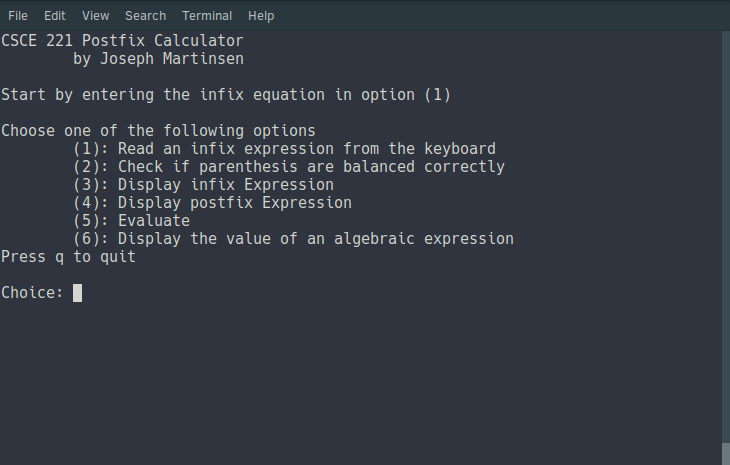
\includegraphics[scale=0.3]{img1.png}
  \end{center}
\end{figure}
\begin{figure}[h]
  \begin{center}
    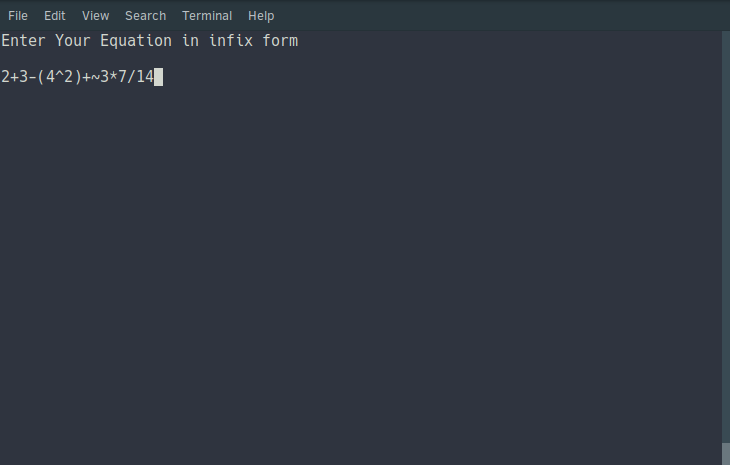
\includegraphics[scale=0.3]{img2.png}
  \end{center}
\end{figure}
\begin{figure}[h]
  \begin{center}
    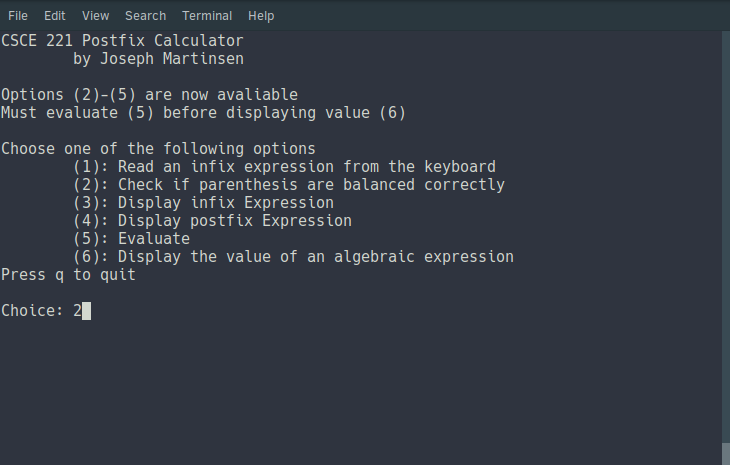
\includegraphics[scale=0.3]{img3.png}
  \end{center}
\end{figure}
\begin{figure}[h]
  \begin{center}
    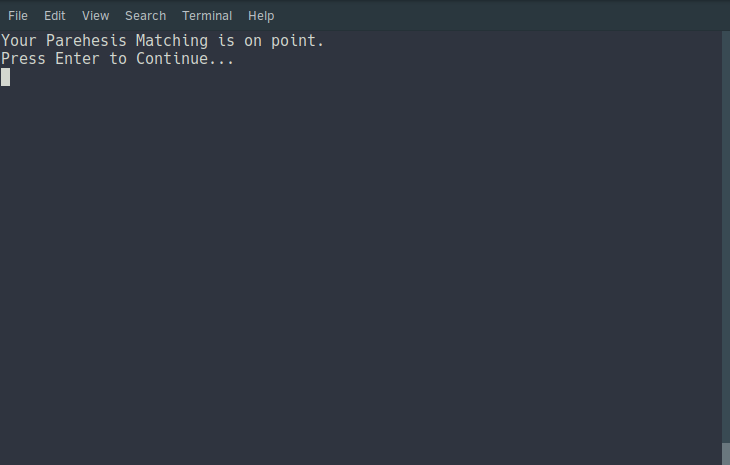
\includegraphics[scale=0.3]{img4.png}
  \end{center}
\end{figure}
\begin{figure}[h]
  \begin{center}
    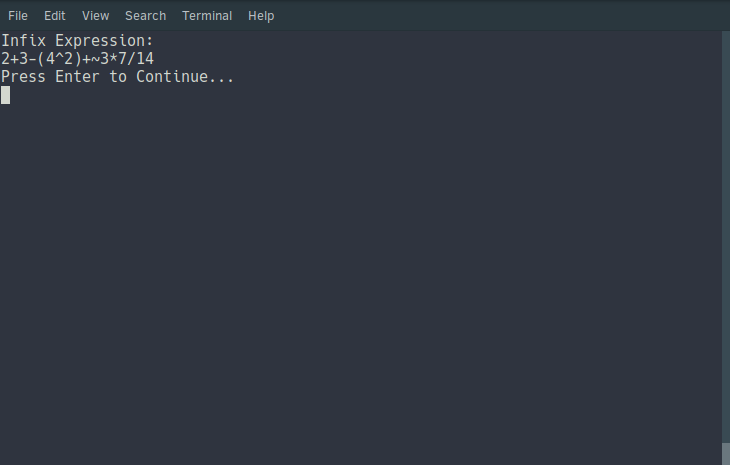
\includegraphics[scale=0.3]{img5.png}
  \end{center}
\end{figure}
\begin{figure}[h]
  \begin{center}
    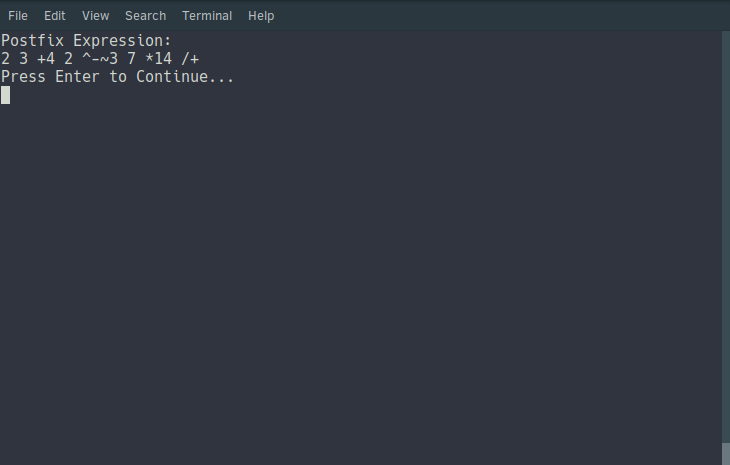
\includegraphics[scale=0.3]{img6.png}
  \end{center}
\end{figure}
\begin{figure}[h]
  \begin{center}
    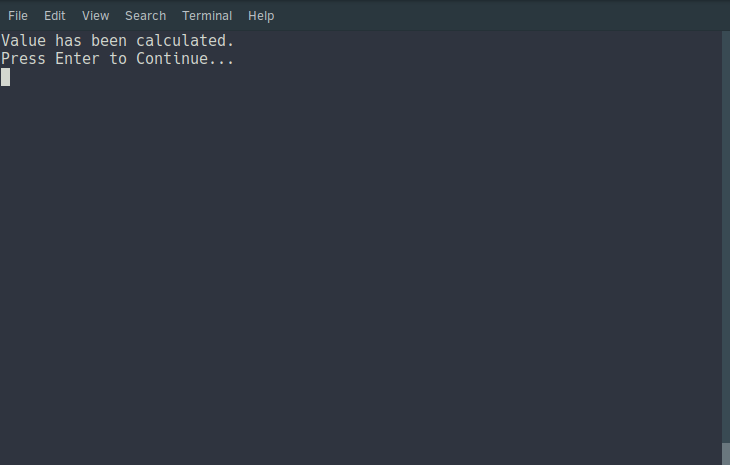
\includegraphics[scale=0.3]{img7.png}
  \end{center}
\end{figure}
\begin{figure}[h]
  \begin{center}
    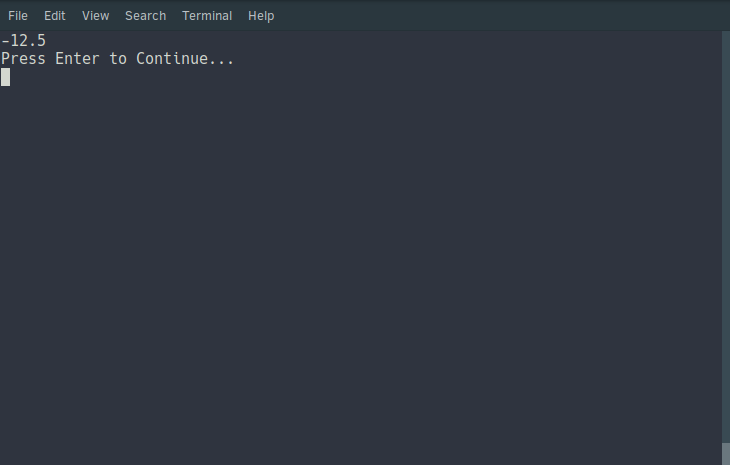
\includegraphics[scale=0.3]{img8.png}
  \end{center}
\end{figure}
\end{enumerate}

\end{document}
